\documentclass{beamer}
%\usepackage{beamerthemeshadow}
\usetheme{Madrid}
\usepackage{color}
\usepackage[all]{xy}

%% Elena's favorite green (thanks, Fernando!)
\definecolor{ForestGreen}{RGB}{34,139,34}
\definecolor{BlueViolet}{RGB}{138,43,226}
\definecolor{Coquelicot}{RGB}{255, 56, 0}
\definecolor{Teal}{RGB}{2,132,130}
%Uncomment this if you want to show work-in-progress comments
\newcommand{\comment}[1]{{\bf \tt  {#1}}}
% Uncomment this if you don't want to show comments
%\newcommand{\comment}[1]{}
% for color names see https://www.overleaf.com/learn/latex/Using_colors_in_LaTeX
\newcommand{\emcomment}[1]{\textcolor{ForestGreen}{\comment{Elena: {#1}}}}

%%%% choose your presentation style:
\mode<presentation>
{
  \usetheme{Copenhagen} %%%
 \usecolortheme{beaver}

%%% set style for ovelays: lists (and other text) appearing one item at a time
%%% This will create a dimmed preview of next item:
%\setbeamercovered{transparent}
%%% This will hide it entirely:
\setbeamercovered{invisible}
}
%% if you don't want page numbers to show: 
\setbeamertemplate{footline}[page number]{}

%%%% 25 minutes time slot, including questions 

\begin{document}
\title{15 Years of Sorting Competitions}
\author{Elena Machkasova}
\institute[UMN Morris] % (optional, but mostly needed)
{
 % \inst{1}%
  University of Minnesota, Morris
}
\date[]  
{Midwest Instruction and Computing Symposium, March 2026}

\begin{frame}
  \titlepage
\end{frame}

%\section{What is a sorting competition?}

\begin{frame}
\frametitle{15 years ago...}
 MICS 2011:
\begin{itemize}
\item Paper on a novel assignment in \textit{Algorithms and Computability} class
\item Typically students implement sorting on numbers and study $O$ efficiency
\item The assignment compared sorting by \textbf{time}
\item Task: sort strings by length, and lexicographically within each length
\item The assignment continued to be offered every year, with a different sorting problem every time
\end{itemize}
\end{frame}

\begin{frame}
 \frametitle{Outline}
\tableofcontents
\end{frame}

\section{Overview and Setup}

\begin{frame}
\frametitle{Why sorting?}
\begin{itemize}
\item No one perfect algorithm - lots of things to try
\item Details matter! - problem solving
\end{itemize}
\qquad\qquad 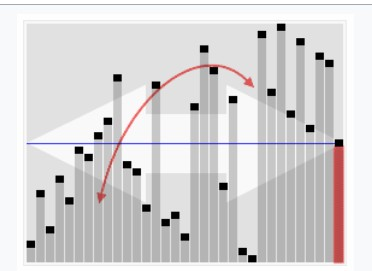
\includegraphics{Quicksort.jpg} \\
\qquad\qquad Source: https://en.wikipedia.org/wiki/Quicksort
\end{frame}

\begin{frame}
\frametitle{Setup (summary)}
\begin{itemize}
\item Programming in Java
\item Timed portion: only sorting
\item Template: file input/output
\item Reference Java implementation: slow, correct
\item Correctness: exact match to the output of reference implementation
\item Data generator, usually with parameters (number of items, length of strings, etc.)
\item Single core run
\item JVM warmup provided
\end{itemize}
\end{frame}

\begin{frame}
\frametitle{Scoring and logistics}
\begin{itemize}
\item 2 preliminary rounds, 1 final round
\item Compiled code (but not source code) is posted after each preliminary round
\item Groups are anonymous, identified by numbers
\item After the final round all source code is posted, groups revealed
\item Each round has 2-3 datasets to sort
\item Each solution is ran 3 times on each dataset, the median time counts
\item Incorrect sorting gets penalty of 1000000ms. 
\end{itemize}
\end{frame}

\section{Sorting Problems}

\begin{frame}
\frametitle{Some past problems (omitting details)}
\begin{itemize}
\item 2014: binary strings to be sorted by length, then by the number of 1s
\item 2016: 2D points on a grid generated as ``walks' to be sorted by the distance to the closest of two  constant points 
\item 2017: positive integers to be sorted by the product of two smallest different prime factors
\item 2021: binary numbers to be sorted by the number of 1s, then by the length of the longest repeated substring
\item 2022: mix of decimal fractions and rational numbers to be sorted  by value.  For equal numbers the decimal representation is considered ``smaller'' than a fraction for positives and ``larger'' for negatives 
\item 2023: Fixed length integers to be sorted by the sum of all unique prime factors. Equal sums are sorted by value in decreasing order
\item 2025: Binary strings of the same length are to be sorted by their distance from a ``target'' string. 
\end{itemize}
\end{frame}

\begin{frame}
\frametitle{Important aspects of problems}
Approaches that are commonly tried (as combinations)
\begin{itemize}
\item Lots of duplicates -- modified quicksort, counting sort, separating into buckets
\item Fixed length -- radix sort
\item Uniform distribution -- variations of bucket sort
\item Ordered subsequences (``walks'') -- mergesort, TimSort, insertion sort
\item Fits into a long -- quicksort or any predefined sort on longs
\item Repeated computations (e.g. finding prime factors) -- storing results
\item Multiple sorting paths -- stable sorting matters, although ``buckets'' are also used
\item Made appearance: heapsort, comb sort, prefix trees,....
\end{itemize}
\end{frame}

\section{Correctness}

\begin{frame}
\frametitle{Correctness review}
A solution is correct if it follows all the rules (memory used, etc.) and produces correct sorting for \textit{any} 
data that can be generated by the data generator.  
\begin{itemize}
\item At the competition: compared to reference representation
\item After the final round: every group is assigned a ``review'' group
\item Extra credit: for anyone reporting a correctness issue in \textbf{any} submission before their ``reviewer'' group does
\item A group not passing correctness review is disqualified
\item Rules decisions need to be made for unusual solutions: multithreading
\end{itemize}
\end{frame}

%\section{Outcomes}

\section{Community Matters}

\begin{frame}
\frametitle{Open competition}
 \begin{itemize}
\item 
\end{itemize}
\end{frame}

\begin{frame}
\frametitle{Presentations}
\begin{itemize}
\item 
\end{itemize}
\end{frame}

\section{Conclusions}

\begin{frame}
\frametitle{Conclusions and the future}

\end{frame}

\begin{frame}
\frametitle{Acknowledgments, more info}

\end{frame}

\end{document}